\documentclass[dvipdfmx]{ujarticle}
\usepackage{eee}

\begin{document}
\title{平成31年 電磁気学II}
\date{}
\author{大山主朗}

\maketitle

\section*{平成31年 電磁気学II 前期中間試験}

\section{以下に示す物理定数は電磁気学を修めた者であれば常識的に覚えていなければならない数値である.それぞれの値を示せ.}
\begin{enumerate}[(a)]
	\item 真空の誘電率$\varepsilon_{0}:8.854 \times 10^{-12}\,\rm{F/m}$
	\item 真空の透磁率$\mu_{0}:1.257 \times 10^{-6}\,\rm{H/m}$
	\item 電子の電荷$e:-1.602 \times 10^{-19}\,\rm{C}$
	\item 電子の静止質量$m:9.109\times 10^{-31}\,\rm{kg}$
\end{enumerate}

\section{$xy$直交座標系において,同量異符号の点磁荷$\pm m$が距離$l$に固定された磁気双極子が存在する.このとき以下の問いに答えよ.}
\begin{enumerate}[(a)]
	\item 点Aに存在する磁荷$-m$が点P$(x_0,y_0)$に作る磁界$H_{1}$を求めよ.また,$H_{1}$を$x$方向成分$H_{x1}$と$y$方向成分$H_{y1}$に分解せよ.
	\begin{align*}
		\boldsymbol{H}_{1}&=\frac{1}{4\pi \mu_{0}}\frac{-m}{\left(\left(x_{0}+\frac{l}{2}\right)^{2}+y_{0}^{2}\right)^{3/2}} \left\{ \left(x_{0}+\frac{l}{2}\right)\boldsymbol{i}+y_{0}\boldsymbol{j}\right\}\,[\rm{A/m}]\\
		|\boldsymbol{H}_{1}|&=\frac{1}{4\pi \mu_{0}}\frac{m}{\left(x_{0}+\frac{l}{2}\right)^{2}+y_{0}^{2}}\,[\rm{A/m}] \\
		|\boldsymbol{H}_{x1}|&=\frac{1}{4\pi \mu_{0}}\frac{m}{\left(\left(x_{0}+\frac{l}{2}\right)^{2}+y_{0}^{2}\right)^{3/2}}\left(x_{0}+\frac{l}{2}\right) \,[\rm{A/m}] \quad x軸上方向\\
		|\boldsymbol{H}_{y1}|&=\frac{1}{4\pi \mu_{0}}\frac{m}{\left(\left(x_{0}+\frac{l}{2}\right)^{2}+y_{0}^{2}\right)^{3/2}}\,y_{0}\,[\rm{A/m}] \quad y軸下方向
	\end{align*}
	\item 点Bに存在する磁荷$+m$が点P$(x_0,y_0)$に作る磁界$H_{2}$を求めよ.また,$H_{2}$を$x$方向成分$H_{x2}$と$y$方向成分$H_{y2}$に分解せよ.
	\begin{align*}
		\boldsymbol{H}_{2}&=\frac{1}{4\pi \mu_{0}}\frac{m}{\left(\left(x_{0}-\frac{l}{2}\right)^{2}+y_{0}^{2}\right)^{3/2}} \left\{ \left(x_{0}-\frac{l}{2}\right)\boldsymbol{i}+y_{0}\boldsymbol{j}\right\}\,[\rm{A/m}]\\
		|\boldsymbol{H}_{2}|&=\frac{1}{4\pi \mu_{0}}\frac{m}{\left(x_{0}-\frac{l}{2}\right)^{2}+y_{0}^{2}}\,[\rm{A/m}] \\
		|\boldsymbol{H}_{x2}|&=\frac{1}{4\pi \mu_{0}}\frac{m}{\left(\left(x_{0}-\frac{l}{2}\right)^{2}+y_{0}^{2}\right)^{3/2}}\left(x_{0}-\frac{l}{2}\right) \,[\rm{A/m}] \quad x軸正方向\\
		|\boldsymbol{H}_{y2}|&=\frac{1}{4\pi \mu_{0}}\frac{m}{\left(\left(x_{0}-\frac{l}{2}\right)^{2}+y_{0}^{2}\right)^{3/2}}\,y_{0}\,[\rm{A/m}] \quad y軸正方向
	\end{align*}
	\item 点Pでの磁界$H$の$x$方向成分$H_{x}$と$y$方向成分$H_{y}$をそれぞれ求めよ.
	\begin{align*}
		|\boldsymbol{H}_{x}|&=|\boldsymbol{H}_{x1}|+|\boldsymbol{H}_{x2}|\\
		&=\frac{m}{4\pi \mu_{0}}\left\{\frac{1}{\left(\left(x_{0}-\frac{l}{2}\right)^{2}+y_{0}^{2}\right)^{3/2}}\left(x_{0}-\frac{l}{2}\right)-\frac{1}{\left(\left(x_{0}+\frac{l}{2}\right)^{2}+y_{0}^{2}\right)^{3/2}}\left(x_{0}+\frac{l}{2}\right)\right\}\,[\rm{A/m}]\\
		|\boldsymbol{H}_{y}|&=|\boldsymbol{H}_{y1}|+|\boldsymbol{H}_{y2}|\\
		&=\frac{m}{4\pi \mu_{0}}y_{0}\left\{\frac{1}{\left(\left(x_{0}-\frac{l}{2}\right)^{2}+y_{0}^{2}\right)^{3/2}}-\frac{1}{\left(\left(x_{0}+\frac{l}{2}\right)^{2}+y_{0}^{2}\right)^{3/2}}\right\}\,[\rm{A/m}]
	\end{align*}
	\item 磁気双極子モーメント$\boldsymbol{M}$の大きさと方向を求めよ.
	\begin{align*}
		\boldsymbol{M}&=m\boldsymbol{l}\\
		&=ml\boldsymbol{i}\,[\rm{Wb\cdot m}]\\
		|\boldsymbol{M}|&=ml\,[\rm{Wb\cdot m}]\quad x軸正方向
	\end{align*}
	\item 点Pが原点Oより十分遠方にあると仮定すると,$\sqrt{(x_{0}-l/2)^{2}+y_{0}^{2}}\simeq \sqrt{x_{0}^{2}+y_{0}^{2}}$及び$\sqrt{(x_{0}+l/2)^{2}+y_{0}^{2}} \simeq \sqrt{x_{0}^{2}+y_{0}^{2}}$と近似できる.このことを用いて(c)にて得た磁界$H_{x}$及び$H_{y}$を簡略化せよ.
	\begin{align*}
		|\boldsymbol{H}_{x}|&\simeq \frac{ml}{4\pi \mu_{0}\left(x_{0}^{2}+y_{0}^{2}\right)^{3/2}}\,[\rm{A/m}] \quad x軸左方向\\
		|\boldsymbol{H}_{y}|&\simeq 0\,[\rm{A/m}]
	\end{align*}
	\item $y$方向に一様な磁界$\boldsymbol{H}_{0}$が存在するとき,磁気双極子にはたらくトルク$T$を求めよ.
	\begin{align*}
		\boldsymbol{T}&=\boldsymbol{M}H_{0}\sin \theta \\
		&=ml\boldsymbol{i}H_0\sin \frac{\pi}{2}\\
		&=mlH_{0}\boldsymbol{i}\\
		|\boldsymbol{T}|&=mlH_{0}\,[\rm{Wb\cdot m}]
	\end{align*}
\end{enumerate}

\section{磁化されていない強磁性体に磁界$H$を外部から印加し,強磁性体内部での磁束密度$B$を観測すると,図3に示すような結果が得られた.このとき,図中の行程1:点$\rm{O}\to$点$\rm{P_{1}}$,行程 2:点$\rm{P_{1}}\to$点$\rm{P_{2}}$,行程3:点$\rm{P_{2}}\to$点$\rm{P_{3}}$,行程4:点$\rm{P_{3}}\to$点P4,行程5:点P4 $\to$点$\rm{P_{5}}$, 行程6:点$\rm{P_{5}}\to$点P6,行程7:点$\rm{P_{6}}\to$点P1の7つの行程に着目して,測定結果を説明せよ.}

\section{強磁性体,弱磁性体,常磁性体,反磁性体の4つの磁性体の性質を,「比透磁率$\mu_{s}$」と「磁化率$\chi$」という2つの語句を両方用いて説明せよ.}
強磁性体は磁化率$\chi$が0よりかなり大きく,透磁率$\mu_{s}$が1よりかなり大きい磁化されやすい磁性体を指す.そのため,印加した磁界と同じ方向に磁化され,その大きさも大きい.

弱磁性体は磁化率$\chi$が0より大きく,透磁率$\mu_{s}$より小さい磁性体である.

常磁性体は磁化率$\chi$が0より大きく,透磁率$\mu_{s}$は1未満の磁性体を指す.そのため,印加した磁界と同じ方向に磁化され,その大きさは大きくない.

反磁性体は磁化率$\chi$が0より小さく,透磁率$\mu_{s}$が1より小さい磁性体を指す.そのため,印加した磁界と逆方向に磁化され,その大きさは小さい.

反磁性体は磁化率$\chi$が0より小さく,透磁率$\mu_{s}$が1より小さい磁性体を指す.そのため,印加した磁界と逆方向に磁化され,その大きさは小さい.

\section{$xyz$直交座標系の$xy$平面内に原点Oを中心する半径$a$の円周状に電流$I$が流れている.このとき,以下の場所に発生する磁界$H$とその方向を求めよ.}
\begin{enumerate}[(a)]
	\item 原点O
	\begin{align*}
	\boldsymbol{H}&=\oint d\boldsymbol{H}\\
	円周上に&線素ベクトルd\boldsymbol{l}をとる.\\
	ここで,円周上のどの点&でもd\boldsymbol{H}の向きが同じなので,\\
	H&=\oint dH\\
	&=\oint \frac{I\sin \theta }{4\pi r^{2}}dl\\
	&=\frac{I\sin \frac{\pi}{2} }{4\pi r^{2}}\cdot 2\pi r\\
	&=\frac{I}{2r}\\
	&=\frac{I}{2a}\,[\rm{A/m}]\quad 上向き
\end{align*}

	\item $(x, y, z)=(0, 0, h)$となる$z$軸上の点P
	\begin{align*}
	y>0に円周上の&微小磁界d\boldsymbol{H}_{1}を\\
	y<0に円周上の&微小磁界d\boldsymbol{H}_{2}を考える.\\
	またそれぞれの&線素ベクトルをd\boldsymbol{l}ととる.\\
	ここで,d\boldsymbol{H}_{1}とd\boldsymbol{H}_{2}の外積より,&2つの磁界は打ち消される方向となっているため,\\
	d\boldsymbol{H}_{1}とd\boldsymbol{H}_{2}を合成した&磁界をd\boldsymbol{H}とする.(\phi:d\boldsymbol{H}_{2}とd\boldsymbol{H}のなす角)\\
	|d\boldsymbol{H}_{1}|=|d\boldsymbol{H}_{2}|&=\frac{Idl}{4\pi r^{2}}\sin \theta\\
	&=\frac{Idl}{4\pi (a^{2}+h^{2})}\\
	d\boldsymbol{H}&=2d\boldsymbol{H}_{1}\cos \phi\\
	&=2d\boldsymbol{H}_{1}\frac{a}{r}\\
	&=2d\boldsymbol{H}_{1}\frac{a}{\sqrt{a^{2}+h^{2}}}\\
	|d\boldsymbol{H}|&=2|d\boldsymbol{H}_{1}|\frac{a}{\sqrt{a^{2}+h^{2}}}\\
	&=\frac{aIdl}{2\pi (a^{2}+h^{2})^{3/2}}\\
	\boldsymbol{H}&=\oint d\boldsymbol{H}_{1}\\
	|\boldsymbol{H}|&=\frac{1}{2}\oint|d\boldsymbol{H}|\\
	&=\frac{1}{2}\oint \frac{aIdl}{2\pi (a^{2}+h^{2})^{3/2}}\\
	&=\frac{1}{2}\cdot \frac{aI}{2\pi (a^{2}+h^{2})^{3/2}} \cdot 2\pi a\\
	&=\frac{a^{2}I}{2 (a^{2}+h^{2})^{3/2}}\,[\rm{A/m}]\quad 上向き
\end{align*}
\end{enumerate}

\section{$xyz$直交座標系の$y$軸に沿って点Aから点Bまで有限長直線電流$I$が流れている.このとき,$x$軸上の点P$(a, 0, 0)$に発生する磁界$H$とその方向を求めよ.また,有限長直線電流$I$が無限長直線電流$I$になった場合,点Pに発生する磁界$H$を求めよ.}
\begin{align*}
	x方向,y方向,z方向の&基底ベクトルをそれぞれ\boldsymbol{i},\boldsymbol{j},\boldsymbol{k}とする\\
	この時&d\boldsymbol{l}=dy\boldsymbol{i}, \boldsymbol{r}=a\boldsymbol{i}-y\boldsymbol{j}\\
	d\boldsymbol{l}\times \boldsymbol{r}&=
	\begin{vmatrix}
	\boldsymbol{i} & \boldsymbol{j} & \boldsymbol{k}\\
	0 &dy & 0\\
	a & -y &0
	\end{vmatrix}
	=dy
	\begin{vmatrix}
	\boldsymbol{i}  & \boldsymbol{k}\\
	a & 0
	\end{vmatrix}
	=-ady\boldsymbol{k}\\
	\boldsymbol{H}&=\int_{C} d\boldsymbol{H}\\
	&=-\int_{C} \frac{aI\boldsymbol{k}}{4\pi(a^{2}+y^{2})^{3/2}}dy\\
	&=-\int_{c_{1}}^{c_{2}} \frac{aI\boldsymbol{k}}{4\pi(a^{2}+y^{2})^{3/2}}dy\\
	h&=a\tan \theta と置換する.\\
	\frac{dh}{d\theta}&=\frac{a}{\cos ^{2}\theta } \quad \therefore dh=\frac{a}{\cos ^{2}\theta }d\theta \\
	また積分範囲は&c_{1}\to c_{2}から\alpha-\frac{\pi}{2} \to \beta -\frac{\pi}{2}に変更される.\\
	&=-\int_{\alpha-\frac{\pi}{2}}^{\beta -\frac{\pi}{2}} \frac{a^{2}I}{4\pi a^{3}(1+\tan^{2}\theta)^{3/2}}\boldsymbol{j} \frac{a}{\cos ^{2}\theta }d\theta\\
	&=-\frac{I}{4\pi} \boldsymbol{k} \int_{\alpha-\frac{\pi}{2}}^{\beta -\frac{\pi}{2}} \frac{1}{(1+\tan^{2}\theta)^{3/2}} \frac{1}{\cos ^{2}\theta }d\theta\\
	&=-\frac{I}{4\pi a} \boldsymbol{k} \int_{\alpha-\frac{\pi}{2}}^{\beta -\frac{\pi}{2}} \frac{1}{(\frac{1}{\cos^{2} \theta })^{3/2}} \frac{1}{\cos ^{2}\theta }d\theta\\
	&=-\frac{I}{4\pi a}  \boldsymbol{k}\int_{\alpha-\frac{\pi}{2}}^{\beta -\frac{\pi}{2}} \cos \theta d \theta \\\
	&=-\frac{I}{4\pi a}\left[\sin \theta  \right]_{\alpha-\frac{\pi}{2}}^{\beta -\frac{\pi}{2}} \boldsymbol{k}\\
	&=-\frac{I}{4\pi a}\left\{\sin \left(\beta -\frac{\pi}{2}\right) -\sin \left(\alpha-\frac{\pi}{2}\right) \right\} \boldsymbol{k}\\
	&=-\frac{I}{4\pi a} \left(-\cos \beta +\cos \alpha \right) \boldsymbol{k}\\
	&=-\frac{I}{4\pi a}\left(\cos \alpha -\cos \beta \right) \boldsymbol{k}\,[\rm{A/m}]\\
	直線電流が無限長である&場合は\\
	\alpha=0,&\beta =\pi であるので\\
	\boldsymbol{H}&=-\frac{I}{4\pi a}\cdot 2 \boldsymbol{k}\\
	&=-\frac{I}{2\pi a} \boldsymbol{k}\,[\rm{A/m}]\\
	|\boldsymbol{H}|&=\frac{I}{2\pi a}\,[\rm{A/m}]\quad  紙を突き刺す方向
	\end{align*}
	
\clearpage
\setcounter{section}{0}
\section*{平成31年 電磁気学II 前期期末試験}

\section{以下に示す物理定数は電磁気学を修めた者であれば常識的に覚えていなければならない数値です.それぞれの値を示してください.お願いします.}
\begin{enumerate}[(a)]
	\item 電子の電荷$e:-1.602 \times 10^{-19}\,\rm{C}$
	\item 真空の誘電率$\varepsilon_{0}:8.854 \times 10^{-12}\,\rm{F/m}$
	\item 真空の透磁率$\mu_{0}:1.257 \times 10^{-6}\,\rm{H/m}$
	\item 電子の静止質量$m:9.109\times 10^{-31}\,\rm{kg}$
\end{enumerate}

\section{\wfig{1}に示すような,断面が半径$a$の円柱状の内導体と,内径$b$,外径$c$の厚みのある円筒 状の外導体を有する無限長同軸ケーブルある.この同軸ケーブルは内導体と外導体はそれぞれの中心軸を共有するように配置されている.いま,内導体に一様な電流$I$を,外導体に内導体とは逆方向に一様な電流$I$を流したとき,内外導体の中心軸に垂直な平面内における中心軸からの距離を$r$としたとき,同軸ケーブルの周囲に発生する磁界$H$をアンペールの法則を用いて導出してください.お願いします.}

\begin{figure}[h]
	\centering
	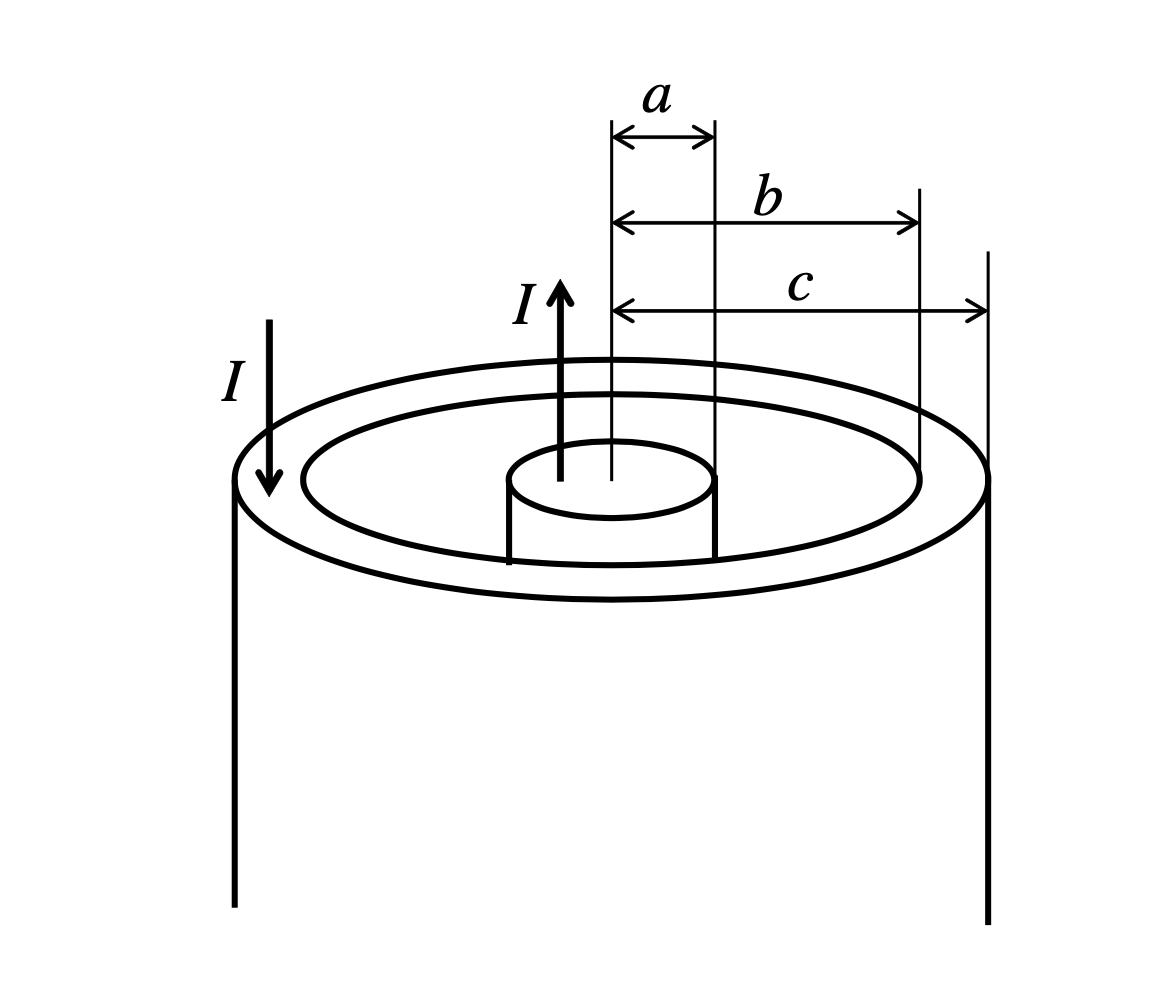
\includegraphics[scale=0.35]{./fig/R03_fig1.png}
	\caption{}
	\label{fig:1}
\end{figure}

\begin{align*}
	r>cのとき&\\
	閉曲面に流れる&電流はI-I=0であるため\\
	H&=0\,[\rm{A/m}]\\
	b<r<cのとき&\\
	dSが上向きである&ことを考慮すると\\
	\int_{C}\boldsymbol{H}\cdot d\boldsymbol{l}&=\int_{C}Hdl=2\pi rH\,[\rm{A}]\\
	\int_{S}\boldsymbol{J}\cdot d\boldsymbol{S}&=\int_{S}JdS=I-\int_{S} \frac{I}{c^{2}\pi-b^{2}\pi}dS\\
	&=I-\frac{I}{c^{2}\pi-b^{2}\pi}\pi(r^{2}-b^{2})=\left(1-\frac{r^{2}-b^{2}}{c^{2}-b^{2}}\right)I\\
	&=\left(\frac{c^{2}-b^{2}-r^{2}+b^{2}}{c^{2}-b^{2}}\right)I=\frac{c^{2}-r^{2}}{c^{2}-b^{2}}I\,[\rm{A}]\\
	2\pi r H&=\frac{c^{2}-r^{2}}{c^{2}-b^{2}}I\\
	H&=\frac{I}{2\pi r}\frac{c^{2}-r^{2}}{c^{2}-b^{2}}\,[\rm{A/m}]\\
	a<r<bのとき&\\
	同様にdSは上向き&とする\\
	\int_{C}\boldsymbol{H}\cdot d\boldsymbol{l}&=\int_{C}Hdl=2\pi rH\,[\rm{A}]\\
	\int_{S}\boldsymbol{J}\cdot d\boldsymbol{S}&=\int_{S} JdS=I\,[\rm{A}]\\
	アンペールの法則より&\\
	H&=\frac{I}{2\pi r}\,[\rm{A/m}]\\
	r<aのとき&\\
	同様にdSは上向き&とする\\
	\int_{C}\boldsymbol{H}\cdot d\boldsymbol{l}&=\int_{C}Hdl=2\pi rH\,[\rm{A}]\\
	\int_{S}\boldsymbol{J}\cdot d\boldsymbol{S}&=\int_{S} JdS=\frac{I}{a^{2}\pi}r^{2}\pi=\frac{r^{2}}{a^{2}}I\,[\rm{A}]\\
	アンペールの法則より&\\
	H&=\frac{\frac{r^{2}}{a^{2}}I}{2\pi r}=\frac{I}{2\pi a^{2}}r\,[\rm{A/m}]\\\\
	\therefore H&=
	\left\{
	\begin{matrix}
	\frac{I}{2\pi a^{2}}r\,[\rm{A/m}] &(0 < r< a)\\\\
	\frac{I}{2\pi r}\,[\rm{A/m}] & (a < r< b) \\\\
	\frac{I}{2\pi r} \frac{c^{2}-r^{2}}{c^{2}-b^{2}}\,[\rm{A/m}] & (b < r <c)\\\\
	0\,[\rm{A/m}] & (r >c)
	\end{matrix}
	\right .  \\
	ただし向きは&左回り(反時計回り)
\end{align*}

\section{\wfig{2}に示すような,単位長さ当たり$n$巻の無限長ソレノイドコイルがある.コイルに電流$I$を流したとき,コイルの周囲に発生する磁界$H$をアンペールの法則を用いて導出してください.お願いします.}

\begin{figure}[h]
	\centering
	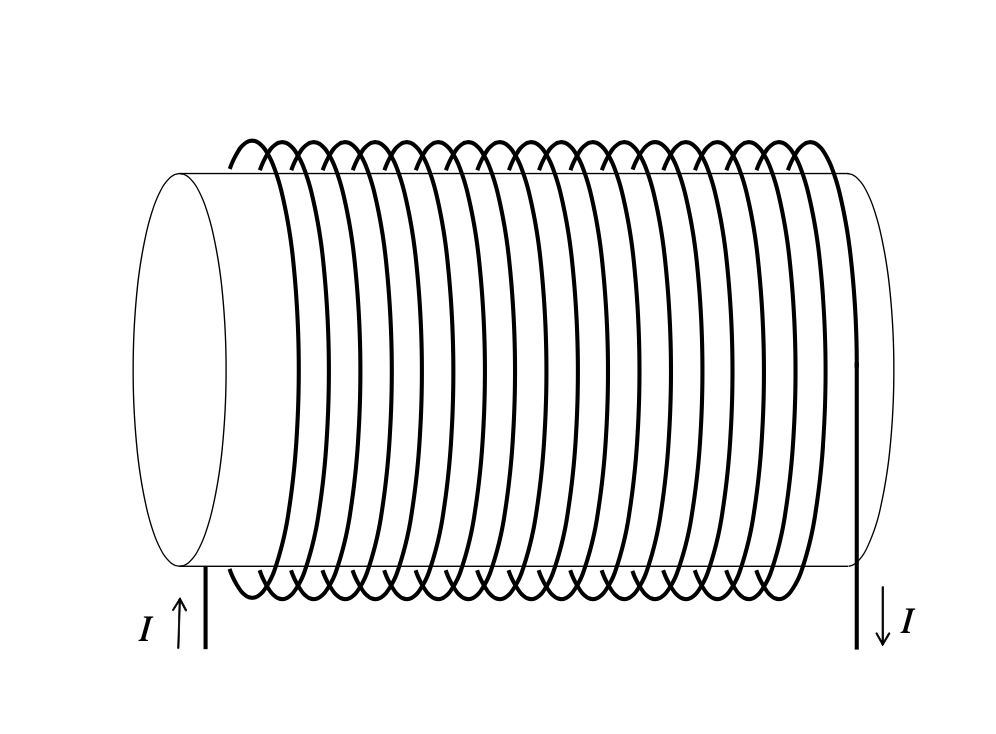
\includegraphics[scale=0.35]{./fig/R03_fig2.png}
	\caption{}
	\label{fig:2}
\end{figure}

\begin{figure}[h]
	\centering
	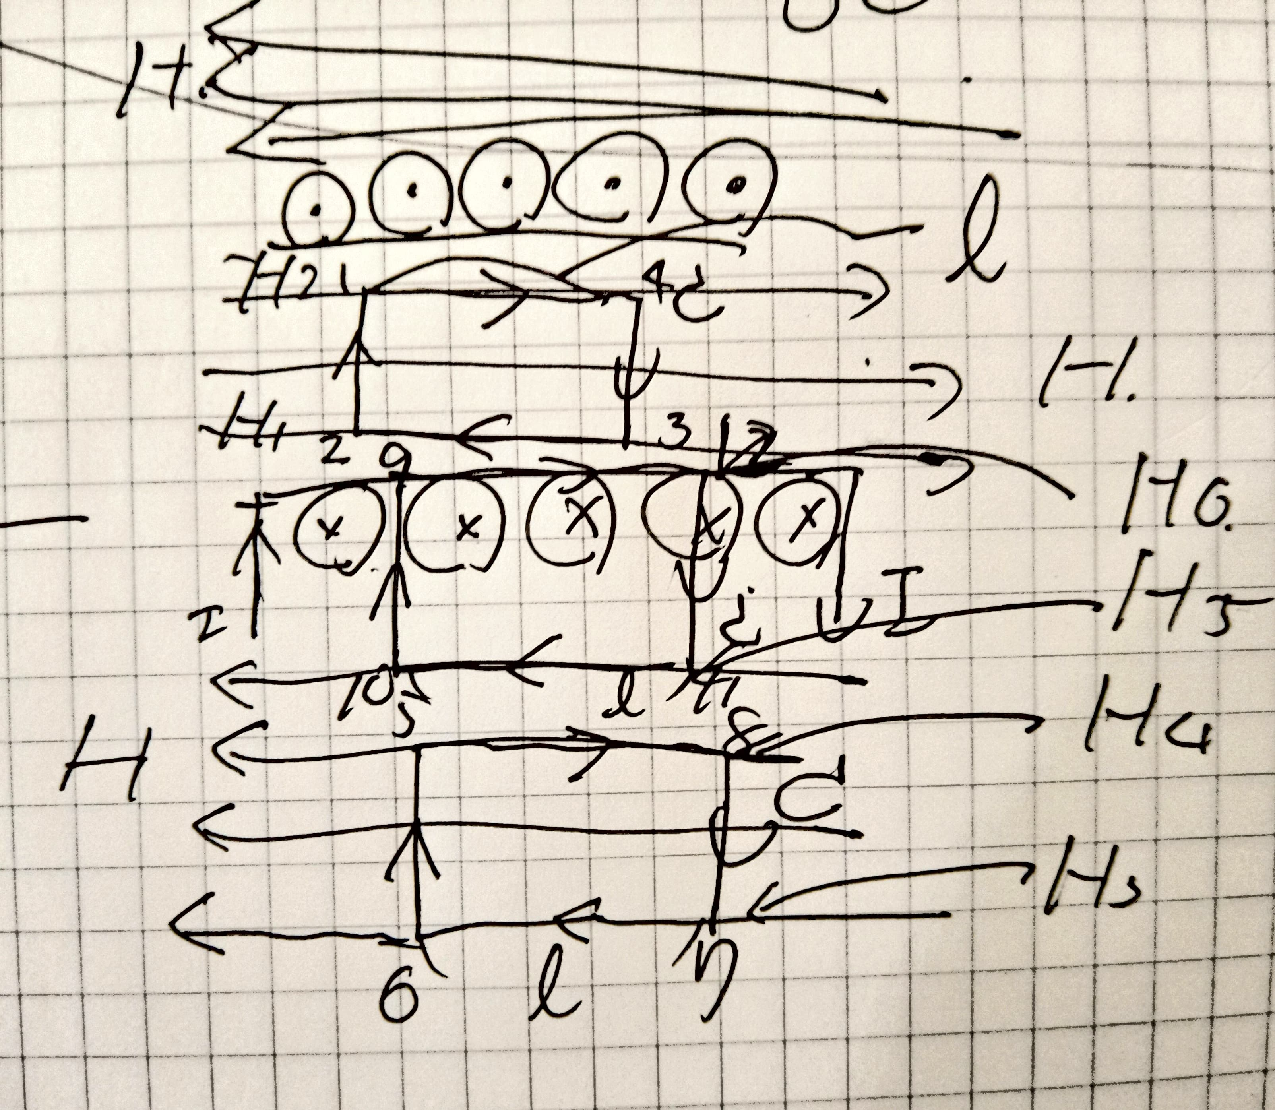
\includegraphics[scale=0.35]{./fig/fig.pdf}
	\caption{}
	\label{fig:a}
\end{figure}


\begin{align*}
このコイルによって発生する磁界はコイル&内部では右向き,コイル外部では左向きとなる.\\
経路Cとしてコイル内に&長方形1234(左上から反時計回りの順)を決める\\
また,経路23上&の磁界をH_{1},経路14上の磁界をH_{2},長さをlとする\\
\int_{C}\boldsymbol{H}\cdot d\boldsymbol{l}&=\int_{12}\boldsymbol{H}\cdot d\boldsymbol{l}+\int_{23}\boldsymbol{H}\cdot d\boldsymbol{l}+\int_{34}\boldsymbol{H}\cdot d\boldsymbol{l}+\int_{41}\boldsymbol{H}\cdot d\boldsymbol{l}\\
\boldsymbol{H}とd\boldsymbol{l}が直交するとき,&内積は0であるため\\
&=\int_{0}^{l}H_{1}dl-\int_{0}^{l}H_{2}dl\\
&=(H_{1}-H_{2})l\,[\rm{A}]\\
\int_{S}\boldsymbol{J}\cdot \boldsymbol{S}&=0\,[\rm{A}]\\
\therefore H_{1}-H_{2}&=0\\
H_{1}&=H_{2}\tag{1}\\
次に経路Cとしてコイル&外部に長方形5678(左上から反時計回りの順)を決める\\
また,経路67上&の磁界をH_{3},経路85上の磁界をH_{4},長さをlとする\\
コイル内の場合と同様の議論により&\\
\int_{C}\boldsymbol{H}\cdot d\boldsymbol{l}&=\int_{56}\boldsymbol{H}\cdot d\boldsymbol{l}+\int_{67}\boldsymbol{H}\cdot d\boldsymbol{l}+\int_{78}\boldsymbol{H}\cdot d\boldsymbol{l}+\int_{85}\boldsymbol{H}\cdot d\boldsymbol{l}\\
\boldsymbol{H}とd\boldsymbol{l}が直交するとき,&内積は0であるため\\
&=-\int_{0}^{l}H_{3}dl+\int_{0}^{l}H_{4}dl\\
&=(H_{4}-H_{3})l\,[\rm{A}]\\
\int_{S}\boldsymbol{J}\cdot \boldsymbol{S}&=0\,[\rm{A}]\\
\therefore H_{4}-H_{3}&=0\\
H_{3}&=H_{4}\\
ここでd \to \infty のときH_{4}&=0\\
\therefore H&=0\,[\rm{A/m}]\left|_{コイル外部}\right .\tag{2}\\
最後に経路Cとしてコイルの境界が経路の中心&となるような長方形9,10,11,12(左上から反時計回りの順)を決める\\
また,経路10,11上&の磁界をH_{5},経路12,9上の磁界をH_{6},長さをlとする\\
今までと同様の議論により&\\
\int_{C}\boldsymbol{H}\cdot d\boldsymbol{l}&=\int_{9,10}\boldsymbol{H}\cdot d\boldsymbol{l}+\int_{10,11}\boldsymbol{H}\cdot d\boldsymbol{l}+\int_{11,12}\boldsymbol{H}\cdot d\boldsymbol{l}+\int_{12,9}\boldsymbol{H}\cdot d\boldsymbol{l}\\
\boldsymbol{H}とd\boldsymbol{l}が直交するとき,&内積は0であり,式(2)よりコイル外部の磁界は0であるため\\
&=H_{5}l\,[\rm{A}]\\
\int_{S}\boldsymbol{J}\cdot \boldsymbol{S}&=\int_{S}JdS=nIl\,[\rm{A}]\\
\therefore H_{5}l&=nIl\\
H_{5}&=nI\,[\rm{A/m}]\\
ここでH_{5}はコイルの内部の磁界であるあるため&式(1)より\\
H&=nI\,[\rm{A/m}]\left|_{コイル内部}\right .
\end{align*}

\section{\wfig{3}に示すように,断面積が半径$r$の円で,比透磁率$\mu_{r}$,半径$R$の円環鉄心に導線を$N$巻したコイルがある.このコイルに電流$I$を流したとき,以下に示す各問いに答えてください.ただし,$r \ll R$とし,発生した磁界はすべて鉄心内部に存在し,漏れ磁界は存在しないものとします.よろしくお願いします.}

\begin{figure}[h]
	\centering
	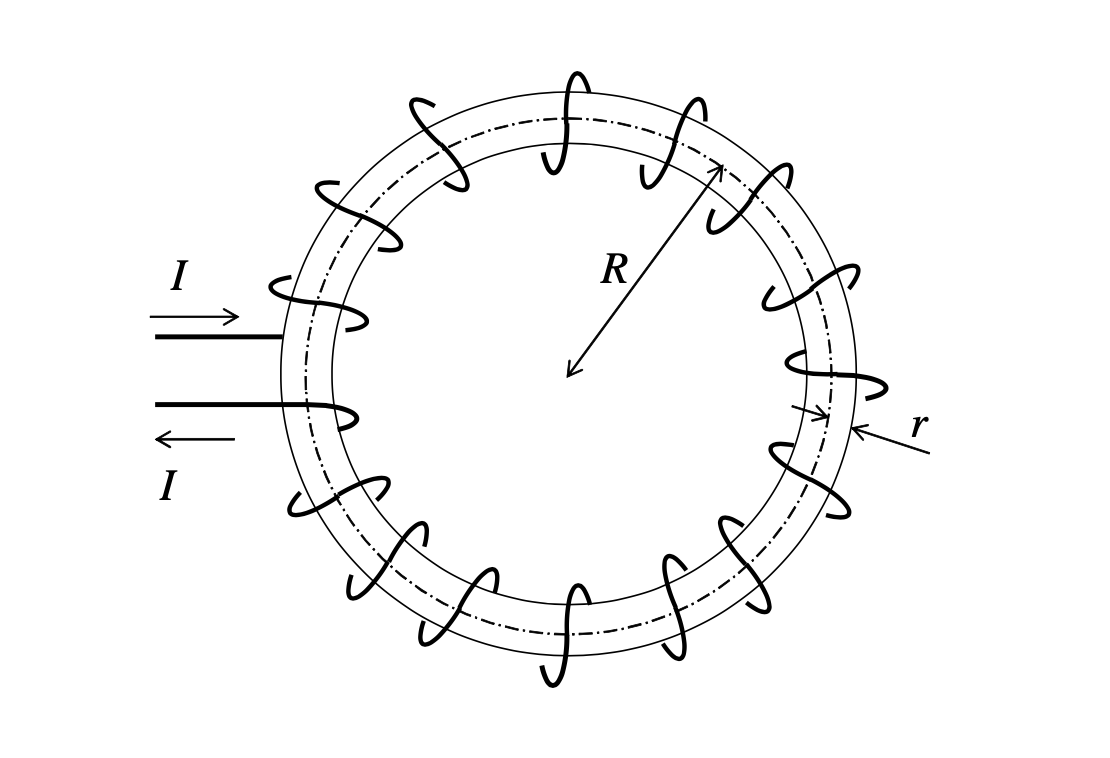
\includegraphics[scale=0.35]{./fig/R03_fig3.png}
	\caption{}
	\label{fig:3}
\end{figure}

\begin{enumerate}[(a)]
	\item 発生する磁界$H$をアンペールの法則を用いて導出してください.お願いします.
	\begin{align*}
	r&\ll Rであるため\\
	\int_{C}\boldsymbol{H}\cdot d\boldsymbol{l}&=\int_{C}Hdl=2\pi RH\,[\rm{A}]\\
	\int_{S}\boldsymbol{J}\cdot d\boldsymbol{S}&=\int_{S}JdS=NI\,[\rm{A}]\\
	\therefore H&=\frac{NI}{2\pi R}\,[\rm{A/m}]
	\end{align*}
	\item 鉄心内部に発生する磁束密度$B$を求めてください.お願いします.
	\begin{equation*}
	B=\mu H=\mu_{0}\mu_{s}H=\frac{\mu_{0}\mu_{s}NI}{2\pi R}\,[\rm{T}]
	\end{equation*}
	\item 鉄心内部に発生する磁束$\Phi$を求めてください.お願いします.
	\begin{equation*}
	\Phi=BS=\frac{\mu_{0}\mu_{s}NI}{2\pi R}\pi r^{2}=\frac{\mu_{0}\mu_{s}r^{2}NI}{2R}\,[\rm{Wb}]
	\end{equation*}
	\item 起磁力を$NI$とすると磁気抵抗$R_{m}$は$R_{m}=\frac{NI}{\Phi}$で求められる.この鉄心の磁気抵抗$R_{m}$を求めてください.お願いします.
	\begin{equation*}
	R_{m}=\frac{NI}{\Phi}=\frac{NI}{\frac{\mu_{0}\mu_{s}r^{2}NI}{2R}}=\frac{2R}{\mu_{0}\mu_{s}r^{2}}\,[\rm{A/Wb}]
	\end{equation*}
\end{enumerate}

\section{An infinitely long tubular conductor has outer radius b and inner radius a offset by a distance c from the axis of the outer cylinder, as shown in figure 4. This eccentric tubular conductor carries a direct current of $I$ amperres. Find the H field at point A shown in the figure. Hint: Consider the tube to be a superposition of two solid cylinders that have radii $b$ and $a$ and that carry uniform current density J in opposite directions.}
Word List\\
infinitely:(adv) 無限に,tubular:(a) 管状の,conductor:(n) 導体,outer:(a) 外の,radius:(n) 半径,inner:(a) 内の,offset:(n) 偏り,distance:(n) 距離,axis:(n) 軸,cylinder:(n) 円筒,fig- ure:(n) 図,eccentric:(a) 偏心的な,direct current:(n) 直流,amperre:(n) アンペア,field:(n) 場・界,consider:(v) 考える,superoposition:(n) 重ね合わせ,solid:(a) 個体,radii:radius の複数形,uniform:(a) 一様な,density:(n) 密度,opposite:(a) 逆の,direction:(n) 方向
\begin{figure}[h]
	\centering
	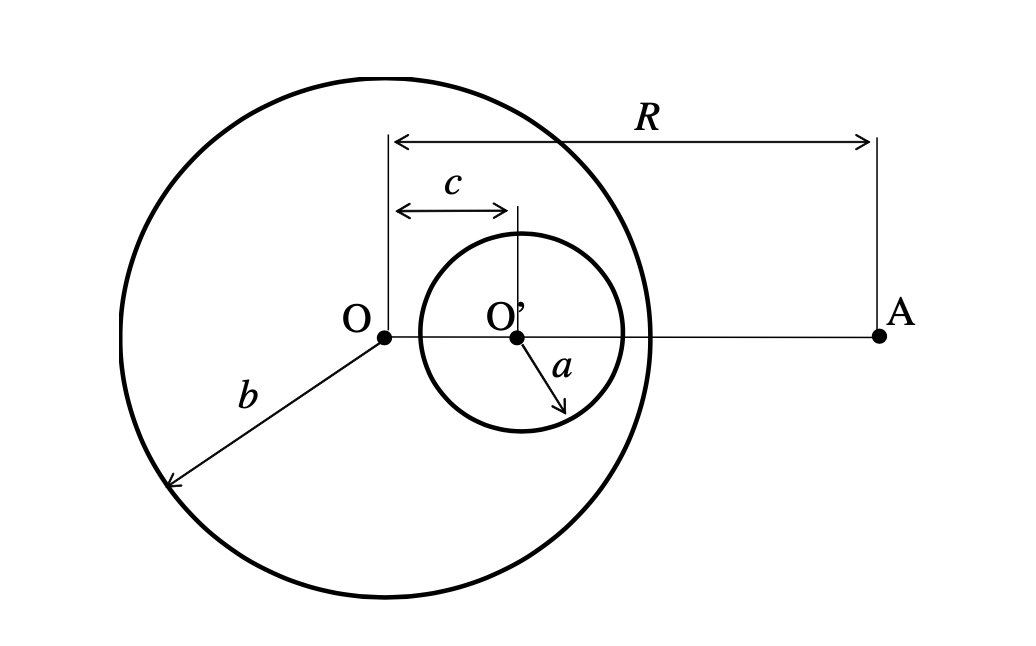
\includegraphics[scale=0.35]{./fig/c.png}
	\caption{}
	\label{fig:c}
\end{figure}

\begin{align*}
	\int_{C}\boldsymbol{H}_{1}\cdot d\boldsymbol{l}&=\int_{C}Hdl=2\pi aH_{1}\,[\rm{A}]\\
	\int_{S}\boldsymbol{J}\cdot d\boldsymbol{S}&=\int_{S}JdS=2\pi (R-c)J\,[\rm{A}]\\
	H_{1}&=\frac{R-c}{a}J\,[\rm{A/m}]\\
	\int_{C}\boldsymbol{H}_{2}\cdot d\boldsymbol{l}&=\int_{C}Hdl=2\pi bH_{2}\,[\rm{A}]\\
	\int_{S}\boldsymbol{J}\cdot d\boldsymbol{S}&=\int_{S}JdS=2\pi RJ\,[\rm{A}]\\
	H_{2}&=\frac{R}{b}J\,[\rm{A/m}]\\
	\text{Because of the point A's Magnetic field that }&\text{this conductor make can disassemble }H_{1}, H_{2}\\
	H&=H_{1}-H_{2}\\
	&=\left(\frac{R-c}{a}-\frac{R}{b}\right)J\,[\rm{A/m}]\quad (a<b)
\end{align*}
\end{document}